% F_rank_scatter: Scatter plot of ISI composite vs rank
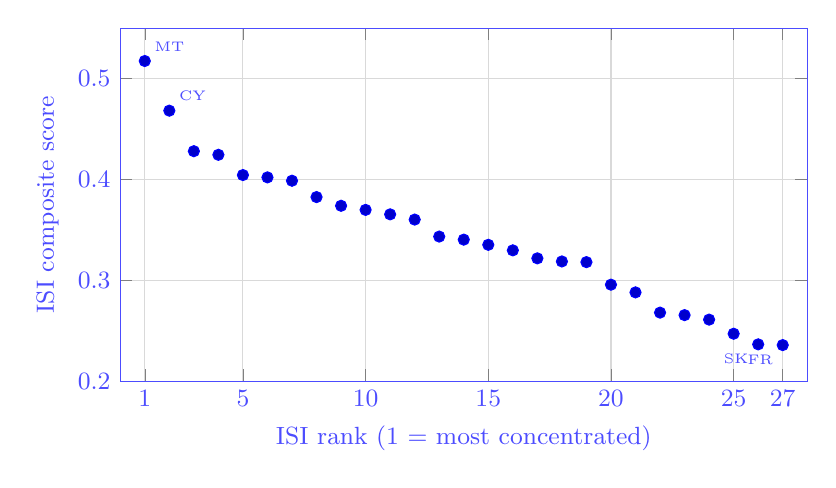
\begin{tikzpicture}
\begin{axis}[
  width=0.85\textwidth,
  height=0.50\textwidth,
  xlabel={ISI rank (1 = most concentrated)},
  ylabel={ISI composite score},
  xmin=0, xmax=28,
  ymin=0.20, ymax=0.55,
  xtick={1,5,10,15,20,25,27},
  grid=major,
  grid style={gray!30},
  tick label style={font=\small},
  label style={font=\small},
  only marks,
  mark=*,
  mark size=2pt,
  blue!70,
]
\addplot coordinates {
  (1, 0.51748148)
  (2, 0.46821264)
  (3, 0.42802519)
  (4, 0.42442738)
  (5, 0.40434768)
  (6, 0.40205136)
  (7, 0.39871532)
  (8, 0.38249806)
  (9, 0.37386086)
  (10, 0.36979186)
  (11, 0.36537350)
  (12, 0.36016893)
  (13, 0.34332177)
  (14, 0.34027984)
  (15, 0.33515702)
  (16, 0.32966227)
  (17, 0.32173430)
  (18, 0.31864192)
  (19, 0.31796630)
  (20, 0.29561321)
  (21, 0.28796781)
  (22, 0.26788694)
  (23, 0.26540520)
  (24, 0.26093977)
  (25, 0.24695137)
  (26, 0.23641567)
  (27, 0.23567126)
};
% Label extremes
\node[font=\tiny, anchor=south west] at (axis cs:1,0.5175) {MT};
\node[font=\tiny, anchor=south west] at (axis cs:2,0.4682) {CY};
\node[font=\tiny, anchor=north east] at (axis cs:27,0.2357) {FR};
\node[font=\tiny, anchor=north east] at (axis cs:26,0.2364) {SK};
\end{axis}
\end{tikzpicture}
